\documentclass[12pt]{article}
\usepackage[utf8]{inputenc}
\usepackage{amsmath}
\usepackage{amsfonts}
\usepackage{amssymb}
\usepackage{empheq}
\usepackage{tikz}
\usepackage{changepage}
\usetikzlibrary{automata, positioning, shapes, arrows}
\addtolength{\topmargin}{-0.875in}
\addtolength{\textheight}{1.75in}

\title{Combinatorics of Integer Partitions}
\author{Ethan Jensen}
\date{February 1, 2019}

\begin{document}
	\maketitle
	\tikzset{
		->, % makes the edges directed
		>=triangle 45, % makes the arrow heads bold
		node distance=3cm, % specifies the minimum distance between two nodes. Change if necessary.
		every state/.style={thick, fill=gray!10}, % sets the properties for each ’state’ node
		initial text=$ $, % sets the text that appears on the start arrow
	}
\definecolor{mycolor1}{RGB}{230,230,230}
\definecolor{mycolor2}{RGB}{210,210,210}
\definecolor{mycolor3}{RGB}{190,190,190}
\section{Condition codes}
\noindent
Recall that \(\mathbb{Z}_+^n\) is defined as
\[\mathbb{Z}_+^n=\{(x_1,x_2,...x_n)|x_1,x_2,...x_n\in\mathbb{Z}_+\}\]
We can define a disjoint partition on \(\mathbb{Z}_+^n\) into subsets based on how elements of the tuple \((x_1,x_2,...x_n)\) are equal to each other.
\newline \newline
\textbf{Definition 1.1.} \textit{Let S be a set of tuples. A \textbf{condition code} C on S is a tuple} \((c_1, c_2,...c_n)\) \textit{that gives S the following elementhood condition:} \newline
\begin{adjustwidth}{2.5em}{0pt}
	\textit{A tuple x is an element of S if and only if there exists a tuple t = \((t_1,t_2,...t_n) \in \mathbb{Z}_+^n\) such that for all i, x contains \(c_i\) copies of \(t_i\).}
\end{adjustwidth}
\(\ \)
\newline
\textbf{Definition 1.2.} \textit{A condition code C is \textbf{spicy} if it gives the following two elementhood conditions:}
\begin{adjustwidth}{2.5em}{0pt}
	\textit{\textbf{(a)} A tuple x is an element of S if and only if there exists a tuple t = \((t_1,t_2,...t_n) \in \mathbb{Z}_+^n\) such that for all i, x contains \(c_i\) copies of \(t_i\).}
	\newline
	\newline
 \textbf{(b) } \textit{Each }\(t_i\)\textit{ is distinct.}
\end{adjustwidth}
\textit{A condition code C that is not spicy is called }\textbf{mild}
\newline
\newline
\textbf{Definition 1.3.} \textit{A condition code C is \textbf{super spicy} if it gives the following two elementhood conditions:}
\begin{adjustwidth}{2.5em}{0pt}
	\textit{\textbf{(a)} A tuple x is an element of S if and only if there exists a tuple t = \((t_1,t_2,...t_n) \in \mathbb{Z}_+^n\) such that for all i, x contains \(c_i\) copies of \(t_i\).}
	\newline
	\newline
 \textbf{(b) } \(t_i\ *< t_{i+1}\) if \(c_i = c_{i+1}\) \textit{ and } \(t_i \neq t_{i+1}\) \textit{ if } \(c_i \neq c_{i+1}\) \textit{where} \((x_n = t_i\) and \(x_m = t_{i+1}) \implies n < m\)
 \newline
 \textit{* Determined to be either} \(>\) \textit{ or } \(<\) \textit{; different for each subset}
\end{adjustwidth}
\(\ \)
\newline
\textbf{Definition 1.4.}
\begin{adjustwidth}{2.5em}{0pt}
	\textbf{(a)}\textit{ A \textbf{mild subset} S of }\(\mathbb{Z}_n^+\)\textit{ written }\(S(c_1)(c_2)...(c_k)\) \textit{ is a subset of }\(\mathbb{Z}_n^+\) \textit{ whose only restrictions on elementhood is a mild condition code.}
	\newline
	\textbf{(b)}\textit{ A \textbf{spicy subset} S of }\(\mathbb{Z}_n^+\)\textit{ written }\(S(c_1,c_2,...c_k)\) \textit{ is a subset of }\(\mathbb{Z}_n^+\) \textit{ whose only restrictions on elementhood is a spicy condition code. S can be identified as a subset of a unique mild subset S'.}
	\newline
	\textbf{(c)}\textit{ A \textbf{super spicy subset} S of \(\mathbb{Z}_n^+\)\textit{ written the same as a spicy subset is a subset of }\(\mathbb{Z}_n^+\) \textit{ whose only restrictions on elementhood is a super spicy condition code. S can be identified as a subset of a unique spicy subset S'.}}
\end{adjustwidth}
\(\ \)
\newline
\textbf{Example 1.1} \newline
Define and ennumerate \(S(1)(1)\), all of its spicy subsets, and their super spicy subsets.
\newline
\(S(1)(1)\) has two spicy subsets - namely \(S(1,1)\) and \(S(2)\). \newline
\(S(1,1)\) has two super spicy subsets. Label them \(S_1(1,1)\) and \(S_2(1,1)\). \newline \(S(2)\) has no super spicy subsets. \newline
From Definition 1.4 we can write \newline
\(S(1)(1)=\{(x_1,x_2)\in \mathbb{Z}_+^2\}=\mathbb{Z}_+^2\) \newline
\(S(1)(1)=\{(1,1),\ (1,3),\ (4,2),\ (1,2),\ (2,3),\ (2,2),\ (3,1)...\}\) \newline \newline
\(S(1,1)=\{(x_1,x_2)\in \mathbb{Z}_+^2 | x_1 \neq x_2\}\) \newline
\(S(1,1)=\{(1,2),\ (2,1),\ (1,6),\ (4,5),\ (3,2)...\}\) \newline
\newline
\(S(2)=\{(x_1,x_2)\in \mathbb{Z}_+^2 | x_1 = x_2\}\) \newline
\(S(2)=\{(1,1),\ (3,3),\ (7,7),\ (4,4)...\}\) \newline
\newline
\(S_2(1,1)=\{(2,1),\ (4,1),\ (4,3),\ (7,5),\ (6,2)...\}\) \newline
\section{A Multi-layered Partition}
Note the following hierarchy:
\begin{itemize}
	\item a mild subset is a subset of \(\mathbb{Z}_+^n\).
	\item a spicy subset is a subset of a mild subset.
	\item a super spicy subset is a subset of a spicy subset.
\end{itemize}
Consider the following diagram
\begin{figure}[ht]
	\centering
	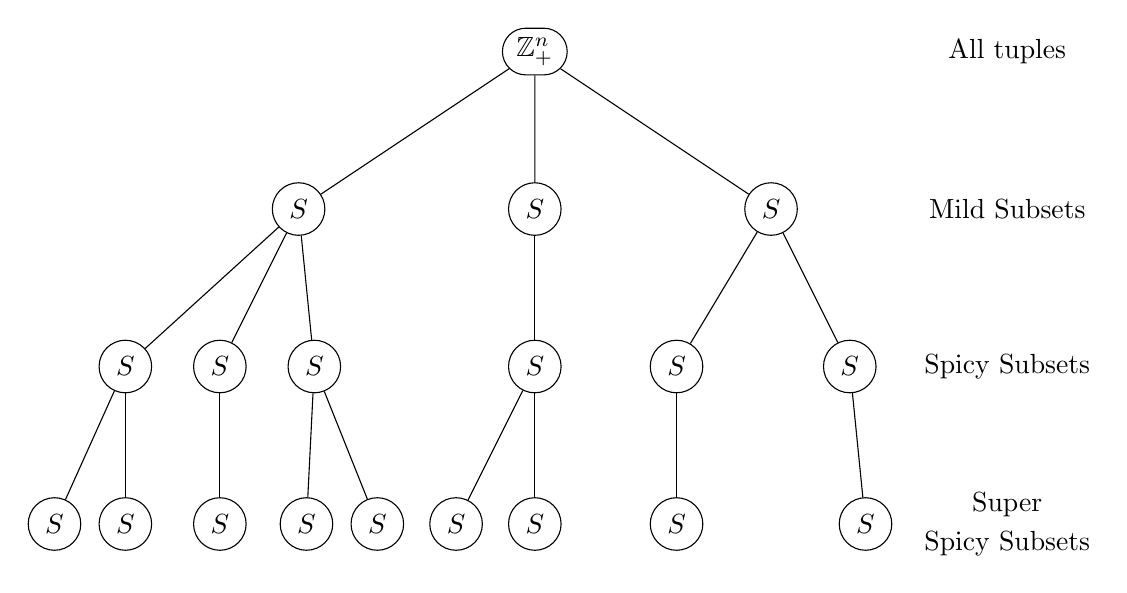
\begin{tikzpicture}
	\node[draw, shape = rounded rectangle] (s0) at (0, 6) {$\mathbb{Z}_+^n $};
	\node[draw, shape = circle] (s1) at (-3, 4) {$ S $};
	\node[draw, shape = circle] (s2) at (0, 4) {$ S $};
	\node[draw, shape = circle] (s3) at (3, 4) {$ S $};

	\node[draw, shape = circle] (s4) at (-5.2, 2) {$ S $};
	\node[draw, shape = circle] (s5) at (-4, 2) {$ S $};
	\node[draw, shape = circle] (s6) at (-2.8, 2) {$ S $};

	\node[draw, shape = circle] (s8) at (0, 2) {$ S $};

	\node[draw, shape = circle] (s10) at (1.8, 2) {$ S $};
	\node[draw, shape = circle] (s12) at (4, 2) {$ S $};

	\node[draw, shape = circle] (s13) at (-6.1, 0) {$ S $};
	\node[draw, shape = circle] (s14) at (-5.2, 0) {$ S $};

	\node[draw, shape = circle] (s15) at (-4, 0) {$ S $};
	\node[draw, shape = circle] (s16) at (-2.9, 0) {$ S $};
	\node[draw, shape = circle] (s17) at (-2, 0) {$ S $};

	\node[draw, shape = circle] (s18) at (-1, 0) {$ S $};
	\node[draw, shape = circle] (s19) at (0, 0) {$ S $};

	\node[draw, shape = circle] (s20) at (1.8, 0) {$ S $};
	\node[draw, shape = circle] (s21) at (4.2, 0) {$ S $};

	\node[] (thing1) at (6,6) {All tuples};
	\node[] (thing1) at (6,4) {Mild Subsets};
	\node[] (thing1) at (6,2) {Spicy Subsets};
	\node[] (thing1) at (6,0.25) {Super};
	\node[] (thing1) at (6,-0.25) {Spicy Subsets};

	\draw
	(s0) edge (s1)
	(s0) edge (s2)
	(s0) edge (s3)

	(s1) edge (s4)
	(s1) edge (s5)
	(s1) edge (s6)

	(s2) edge (s8)

	(s3) edge (s10)
	(s3) edge (s12)

	(s4) edge (s13)
	(s4) edge (s14)

	(s5) edge (s15)

	(s6) edge (s16)
	(s6) edge (s17)

	(s8) edge (s18)
	(s8) edge (s19)

	(s10) edge (s20)
	(s12) edge (s21);

	\end{tikzpicture}
	\caption{Partition Diagram}
\end{figure}
\newline
\textbf{Lemma 1.1.} \textit{Two condition codes are equivalent if they are permutations of each other.} \newline
\textbf{Proof.}
Consider any two condition codes \(C_1=(a_1,a_2,...a_n)\) and \(C_2=(b_1,b_2,...b_n)\) which are permutations of each other.
\newline
Assume some \(x \in S(C_1)\).
\newline
By Definition 1.1, a tuple x is an element in \(S(C_1)\) if for all i, there exists a tuple \((t_1,t_2,...t_n)\in \mathbb{Z}_n^+\) such that x contains \(a_i\) copies of \(t_i\). \newline
\newline
Applying the assumed permutation, there exists \((s_1,s_2,...s_n)\in \mathbb{Z}_n^+\) such that for all i, x contains \(b_i\) copies of \(s_i\).
\newline
\newline
Thus, \(x \in S(C_2)\) and \(S(C_2) \subseteq S(C_1)\).
\newline
The same process can be done to show that \(S(C_1) \subseteq S(C_2)\).
\newline
\(\therefore S(C_1) = S(C_2)\) and the condition codes are equivalent.
\newline \(\blacksquare\) \newline \newline
\textbf{Theorem 1.1.} \textit{The set of all super spicy subsets S with distinct condition codes C of} \(\mathbb{Z}_n^+\) \textit{forms a disjoint partition of \(\mathbb{Z}_n^+\).} \newline \newline
\textbf{Proof. } Show that each distinct set is disjoint. \newline
\newline
Consider any two distinct super spicy subsets \(S(C_1)\) and \(S(C_2)\),
where \newline
\(C_1=(a_1,a_2,...a_k),\ C_2=(b_1,b_2,...b_k)\)\newline
Suppose \(x\in S(C_1)\cap S(C_2)\). \newline
\(\exists (t_1,t_2,...t_k) \ni\) x contains \(a_i\) copies of \(t_i\) for all i. \newline
\(\exists (s_1,s_2,..s_k) \ni\) x contains \(b_i\) copies of \(s_i\) for all i.
\newline
This implies that \((t_1,t_2,...t_k)\) is a permutation of \((s_1,s_2,..s_k)\). \newline
This further implies that \(C_1=(a_1,a_2,...a_k),\ C_2=(b_1,b_2,...b_k)\) are permutations of each other and are equivalent by Lemma 1.1.\newline
This is a contradiction. \newline
Thus, there is no \(x\in S(C_1)\cap S(C_2)\).
\newline
\(S(C_1)\cap S(C_2) = \varnothing\)
\newline \(\square\) \newline
Show that \(\bigcup P =\mathbb{Z}_+^n\), where P is the set of all spicy subsets.
\newline
\newline
\(S\in P \implies S \subseteq \mathbb{Z}_+^n\) by definition. So \(\bigcup P \subseteq \mathbb{Z}_+^n\).
\newline
Assume \(x = (x_1,x_2,...x_n) \in \mathbb{Z}_+^n\).
\newline
Let \(a_i\) be the first occurence of \(x_i\) in x.
\newline
Consider the tuple \((a_1,a_2,...a_k)\) each of whose values are distinct values in x and \(x_n = a_i\) and \(x_m = a_{i+1} \implies n < m\)
\newline
There exists some spicy condition code \(C=(c_1,c_2,...c_k)\) such that x contains \(c_i\) copies of \(a_i\) for all i.
\newline
By Definition 1.2, \(x \in S(C) \in P\) where P is the collection of all spicy subsets.
\newline
by the Union Lemma, \(x \in \bigcup P\)
\newline
\(\mathbb{Z}_+^n \subseteq \bigcup P\)
\newline
\(\therefore \bigcup P = \mathbb{Z}_+^n\)
\newline \(\blacksquare\) \newline \newline
\textbf{Example 1.2} \newline
Show that Theorem 1.1 holds for \(S(1)(1)\), and all if its super spicy subsets. \newline \newline
As seen in Example 1.1, the spicy subsets for \(S(1)(1)\) are \(S(1,1) and S(2)\), where \newline
\(S(1,1)=\{(x_1,x_2)\in \mathbb{Z}_+^2 | x_1 \neq x_2\}\) \newline
\newline
\(S(2)=\{(x_1,x_2)\in \mathbb{Z}_+^2 | x_1 = x_2\}\) \newline
It is easy to see by the elementhood conditions for these two sets that they form a disjoint partition of \(S(1)(1)\).
\newline \newline
As seen in Example 1.1, thew spicy subsets for \(S(1)(1)\) are
\newline
\(S_1(1,1)=\{(x_1,x_2)\in \mathbb{Z}_+^2 | x_1 < x_2\}\) \newline
\newline
\(S_2(1,1)=\{(x_1,x_2)\in \mathbb{Z}_+^2 | x_1 > x_2\}\) \newline
Once again, it is easy to see that these two subsets form a disjoint partition of their superset, \(S(1,1)\). \newline
\newline
This verifies Theorem 1.1 for \(S(1)(1)\). \newline
\section{The D function}
The fact that the spicy subsets form a disjoint partition of \(\mathbb{Z}_+^n\) means that linear functions on the set \(\mathbb{Z}_+^n\) can instead be applied on each of the spicy subsets instead to get the same result.
\newline \newline
In particular, a new function can be defined called the D function, which when combined with this disjoint partition, can take a simple trigonometric identity and use it to calculate difficult infinite sums.
\newline \newline
\textbf{Definition 1.5.} \textit{Let } \(x = (x_1,x_2,...x_n)\in \mathbb{Z}_+^n\)\textit{ and S(C) be a mild subset or a super spicy subset.}
\newline
\textit{Define }\(D:C\rightarrow \mathbb{R}\) \textit{ by }
\[\sum_{x \in S(C)}\frac{1}{(x_1)^2}\frac{1}{(x_2)^2}...\frac{1}{(x_n)^2}=\sum_{x \in S(C)}\prod_{x_i}x_i^{-2}\]
\textit{For a mild condition code we write: }\(D(c_1)(c_2)...(c_n)\)
\newline
\textit{For a super spicy condition code we write: }\(D(c_1,c_2...c_n)\)
\newline \newline
\textbf{Definition 1.6} \newline
\textit{Let} \(D_n(a)\) \textit{represent} \(\overbrace{D(a,a,...a)}^{n}\)
\newline
\textit{Let} \(D^n(a)\) \textit{represent} \(\overbrace{D(a)(a)...(a)}^{n}\)
\newline
\newline
\textbf{Theorem 1.2}\newline
\(D(C_1)D(C_2)=D(C_1)(C_2)\) \newline
\newline
\textbf{Proof.} By Definition 1.5. , we can write
\[D(C_1)(C_2) =\sum_{x\in S(C_1)}\prod_{x_i}x_i^{-2}\sum_{y\in S(C_2)}\prod_{y_i}y_i^{-2}\]
\[D(C_1)(C_2) =\sum_{x\in S(C_1)}\sum_{y\in S(C_2)}\prod_{x_i}x_i^{-2}\prod_{y_i}y_i^{-2}\]
Let \(z = (x | y)\) such that
\[z = (x_1,x_2,x_3,...x_n,y_1,y_2,y_3...y_m)\]
Then by Definition 1.1, just combining elementhood conditions together,
\[D(C_1)D(C_2) =\sum_{z \in S(C_1)(C_2)}\prod_{Z_i}z_i^{-2}\]
\[\therefore D(C_1)D(C_2) = D(C_1)(C_2)\]
\(\blacksquare\)
\newline
\newline
\textbf{Theorem 1.3} \(D_n(1)=\frac{\pi^{2n}}{(2n+1)!}\)
\newline
\textbf{Proof.}\newline
Compare the MacLaurin series of \(\sinh(x)\) with the Euler product of \(\sinh(x)\).
\[\sinh(x)=\frac{x}{1!} + \frac{x^3}{3!} + \frac{x^5}{5!} + \frac{x^7}{7!}... =x\left(1+\frac{x}{i\pi}\right)\left(1-\frac{x}{i\pi}\right)\left(1+\frac{x}{2i\pi}\right)\left(1-\frac{x}{2i\pi}\right)...\]
Thus, by a simple calculation,
\[\frac{\sinh(\pi x)}{\pi x}=1+\frac{\pi^2x^2}{3!}+\frac{\pi^4x^4}{5!}+\frac{\pi^6x^6}{7!}...=\left(1+\frac{x^2}{1^2}\right)\left(1+\frac{x^2}{2^2}\right)\left(1+\frac{x^2}{3^2}\right)...\]
\newline
When multiplying a product, to calculate the coefficient on a polynomial of the nth degree, all term combinations resulting in the nth degree of each factor must be determined and subsequently summed. \newline
\newline
For the product expansion, the only term combinations resulting in degree 2 are when we select one \(x^2\) term from one factor and select a 1 from each of the other factors. Comparing this to the right hand side we have
\[\frac{\pi^2}{3!}=\frac{1}{1^2}+\frac{1}{2^2}+\frac{1}{3^2}+\frac{1}{4^2}...=D(1)\]
\newline
\newline
Continuing this process we find that
\[\sum_i\sum_{j<i}\frac{1}{i^2}\frac{1}{j^2}=D(1,1)=\frac{\pi^4}{5!}\]
And in general,
\[\sum_{0<x_1}\sum_{x_2<x_1}...\sum_{x_n<x_{n-1}}\frac{1}{x_1^2}\frac{1}{x_2^2}...\frac{1}{x_n^2}=D_n(1)=\frac{\pi^{2n}}{(2n+1)!}\]
\(\blacksquare\)
\newline
\newline
\textbf{Theorem 1.4} \textit{Let } \(C\) \textit{ be a mild condition code and } \(P\) \textit{ be the collection of all super spicy condition codes } \(C_i\) \textit{ where all }\(S(C_i)\subseteq S(C)\).\textit{ Then } \[D(C)=\sum_{C_i\in P}D(C_i)\]
\textbf{Proof. }
\newline
\(\mathbb{Z}_+^n\) has a disjoint parition into super spicy subsets by Theorem 1.2. \newline
Since all super spicy subsets are subsets of mild subsets, every mild subset has a disjoint partion into super spicy subsets.
\newline
\newline
The sum over any set is always equal to the sum over each subset of a disjoint partition.
\newline
Let \(x = (x_1,x_2,...x_n)\in \mathbb{Z}_+^n\), \(C\) be a mild condition code, and each \(C_k\) be super spicy condition codes.
\[\sum_{x \in S(C)}\prod_{x_i}x_i^{-2}=\sum_{S(C_k)\subseteq S(C)}\sum_{x \in S(C_k)}\prod_{x_i}x_i^{-2}\]
\[\therefore D(C)=\sum_{C_i\in P}D(C_i)\]
\(\blacksquare\) \newline
\newpage
\section{Calculating positive even zeta values}
Zeta values can be calculated using disjoint partitions. However, we must prove one more theorem to connect zeta values to the zeta function. \newline \newline
\textbf{Theorem 1.5} \(D(n) = \zeta(2n)\)\textit{ for } \(n=1,2,3...\) \newline \newline
We define \(\zeta(s)\) to be \(\zeta(s) = \sum_{k=1}^{\infty}\frac{1}{k^s}\). \newline
By Definition 1.4 we see that any mild subset \(S(C)\) where C = (n) is a set that only contains tuples of the form \((x_1,x_1,x_1,...), x_1\in \mathbb{Z_+}\) where each element in the tuple is the same. \newline
By Definition 1.5 we can write
\[D(n)=\sum_{x\in S(C)}\prod_{x_i}x_i^{-2}=\sum_{x\in S(C)}x_i^{-2n}\]
The set of all \(x_i\) is just the set of positive integers. Thus,
\[D(n)=\sum_{k=1}^{\infty}\frac{1}{k^{2n}}=\zeta(2n)\]
\(\blacksquare\) \newline \newline
Notice that because of how the D function is defined, only positive even zeta values can be expressed in terms of the D function.
\newline \newline
\textbf{Example 1.3} \newline
From Theorem 1.5 we can express \(\zeta(4)\) in terms of a D function.
\[\zeta(4) = D(2)\]
Using our results from Example 1.2 and Theorem 1.4 we can write
\[D(1)(1) = D_1(1,1) + D_2(1,1) + D(2)\]
where \(D_1(1,1)\) and \(D_2(1,1)\) come from the super spicy subsets \(S_1(1,1)\) and \(S_2(1,1)\) respectively.
\newline \newline
Since \(D_1(1,1)\) and \(D_2(1,1)\) have the same value, we can write
\[D(1)(1) = 2D(1,1) + D(2)\]
From Theorem 1.3, we know that \(D(1)=\frac{\pi^2}{6}\) and \(D(1,1)=\frac{\pi^4}{120}\). \newline
Plugging in these values and using Theorem 1.2 we have
\[\frac{\pi^4}{36}=\frac{\pi^4}{60} + D(2)\]
\[\therefore \zeta(4) = D(2) = \frac{\pi^4}{36}-\frac{\pi^4}{60}=\frac{\pi^4}{90}\]

\newpage
\section{An Example}
\textbf{Ex.} Using disjoint partitions, calculate \(\zeta(8)\)
\newline
Assume \(\zeta(2)=\frac{\pi^2}{6},\ \ \zeta(4)=\frac{\pi^4}{90},\ \ \zeta(6)=\frac{\pi^6}{945}\) \newline \newline
Using Theorem 1.4 we can establish the first 4 equations. \newline
\textbf{(1)} \(D(1)(1)(1)(1) = 24D(1,1,1,1)+12D(1,1,2)+6D(2,2)+4D(1,3)+D(4)\)
\newline
\textbf{(2)} \(D(1)(1)(2) = 2D(1,1,2) + 2D(2,2) + 2D(1,3) + D(4)\)
\newline
\textbf{(3)} \(D(2)(2) = 2D(2,2) + D(4)\)
\newline
\textbf{(4)} \(D(1)(3) = D(1,3) + D(4)\)
\newline \newline
Plugging \textbf{(2)} into \textbf{(1)}
\newline
\textbf{(5)}\ \(D(1)(1)(1)(1) = 24D(1,1,1,1) + 6D(1)(1)(2) - 6D(2,2) - 8D(1,3) -5D(4)\)
\newline
Plugging \textbf{(3)} into \textbf{(5)}
\newline
\textbf{(6)}\ \(D(1)(1)(1)(1) = 24D(1,1,1,1) + 6D(1)(1)(2) - 3D(2)(2) - 8D(1,3) -2D(4)\)
\newline
Plugging \textbf{(4)} into \textbf{(6)}
\newline
\textbf{(7)}\ \(D(1)(1)(1)(1) = 24D(1,1,1,1) + 6D(1)(1)(2) - 3D(2)(2) - 8D(1)(3) +6D(4)\)
\newline
\newline
Using Theorem 1.2 we can write
\newline
\textbf{(8)}\ \((D(1))^4=24D(1,1,1,1)+6(D(1))^2(D(2))-3(D(2))^2-8(D(1))(D(3))+6D(4)\) \newline
Using Theorem 1.3 and Theorem 1.5 we can write \newline
\textbf{(9)}\ \(\zeta(2)^4=24\left(\frac{\pi^8}{9!}\right)+6\zeta(2)^2\zeta(4)-3\zeta(4)^2-8\zeta(2)\zeta(6)+6\zeta(8)\)
\newline
Plugging in \(\zeta(2)=\frac{\pi^2}{6},\ \ \zeta(4)=\frac{\pi^4}{90},\ \ \zeta(6)=\frac{\pi^6}{945}\) we have
\newline
\textbf{(10)}\ \(\frac{\pi^8}{1296}=\frac{\pi^8}{15120}+\frac{\pi^8}{540}-\frac{\pi^8}{2700}-\frac{4\pi^8}{2835}+6\zeta(8)\)
\newline
Isolating \(\zeta(8)\) we have \newline
\textbf{(11)}\ \(\zeta(8)=\frac{1}{6}\left(\frac{\pi^8}{1296}-\frac{\pi^8}{15120}-\frac{\pi^8}{540}+\frac{\pi^8}{2700}+\frac{4\pi^8}{2835}\right)\)
\newline \newline
\boxed{\zeta(8)=\frac{\pi^8}{9450}}
\newpage
\section{Counting spicy subsets}
In the previous example, we have said that
\[D(1)(1)(2) = 2D(1,1,2) + 2D(2,2) + 2D(1,3) + D(4)\]
However, Theorem 1.4 would seem to suggest that
\[D(1)(1)(2) = D(1,1,2) + D(2,2) + D(1,3) + D(4)\]
This equation would be true if each term on the left represented a sum over a spicy subset. However, the notation we use for the D function represents a sum over super spicy subsets.
\newline \newline
If two super spicy subsets \(S(C_1)\) and \(S(C_2)\) are both subsets of the same spicy subset, then \(D(C_1)=D(C_2)\). Thus, all that is left to do is determine the coefficients by determining how many of each category of distinct super spicy subsets are contained in a particular mild subset.
\newline \newline
This turns out to be a non-trivial combinatorics problem. This problem is analagous to determine all the possible ways a given set of blocks can be placed in a given set of holes. \newline
This problem is called the \textbf{Blocks and Holes Problem}.
\begin{figure}[ht]
	\centering % centers the figure
	\begin{tikzpicture}[inner sep=3mm]
\node[draw,fill=mycolor1] (B1) at (0,0) {};
\node[draw,fill=mycolor1] (B2) at (1,0) {};
\node[draw,fill=mycolor1] (B3) at (2,0) {};
\node[draw,fill=mycolor1] (B4) at (2,0.6) {};
\node[] (L1) at (0,-0.6) {$B_1$};
\node[] (L1) at (1,-0.6) {$B_2$};
\node[] (L1) at (2,-0.6) {$B_3$};
\node[] (L1) at (1,1.8) {Blocks};
\node[] (L1) at (4.5,1.8) {Holes};
\node[] (L1) at (4,0) {$H_1$};
\node[] (L1) at (5,0) {$H_2$};
\node[draw,fill=mycolor2,dashed] (H1) at (4,-0.6) {};
\node[draw,fill=mycolor2,dashed] (H2) at (5,-0.6) {};
\node[draw,fill=mycolor2,dashed] (H3) at (5,-1.2) {};
\node[draw,fill=mycolor2,dashed] (H4) at (5,-1.8) {};
\end{tikzpicture}
	\caption{Blocks and Holes Scenario 1.1}
\end{figure}
\begin{figure}[ht]
	\centering % centers the figure
	\begin{tikzpicture}[inner sep=3mm]
	\node[draw,fill=mycolor1] (B1) at (0,0) {};
	\node[draw,fill=mycolor1] (B2) at (1.5,0) {};
	\filldraw[fill=mycolor1] (1.8,-0.3) rectangle (1.2,-1.5);
	\node[] (L1) at (0.6,0) {$B_1$};
	\node[] (L1) at (2.1,0) {$B_2$};
	\node[] (L1) at (2.1,-0.6) {$B_3$};
	\node[] (L1) at (1,1.5) {1};
	\node[] (L1) at (4.5,1.5) {2};

	\node[draw,fill=mycolor1] (B1) at (3.5,0) {};
	\node[draw,fill=mycolor1] (B2) at (5,0) {};
	\filldraw[fill=mycolor1] (5.3,-0.3) rectangle (4.7,-1.5);
	\node[] (L1) at (4.1,0) {$B_2$};
	\node[] (L1) at (5.6,0) {$B_1$};
	\node[] (L1) at (5.6,-0.6) {$B_3$};

	\end{tikzpicture}
	\caption{Blocks and Holes Solution 1.1}
\end{figure}
\newline
The above problem and solution shows that the mild subset S(1)(1)(2) contains exactly 2 super spicy subsets that are subsets of the spicy subset S(1,3).
\newpage
\section{References}
\(\ \)
\newline
“Growth and Change in Mathematics.” Understanding Infinity: the Mathematics of Infinite Processes, by A. Gardiner, Dover Publications, 2002, pp. 19–23.
\newline
\newline
Flammable Maths, "The Basel Problem \& its Alternating Formulation [ The Dirichlet Eta Function ]",\textit{YouTube} video, 15:12. Jan. 11, 2019. \newline
https://www.youtube.com/watch?v=MAoI\_\_hbdWM
\newline
\newline
Flammable Maths, "\textbf{BUT HOW DID EULER DO IT}?! A BEAUTIFUL Solution to the FAMOUS Basel Problem!",\textit{YouTube} video, 18:04. May 24, 2019. https://www.youtube.com/watch?v=JAr512hLsEU
\end{document}
